\chapter{Análise de Resultados}

\section{Interface do usuário}
\begin{figure}[htb]
    \centering
    \caption{Variações de temas da interface principal}
    \label{fig:temas_interface}
    
    \begin{subfigure}{0.9\textwidth}
        \centering
        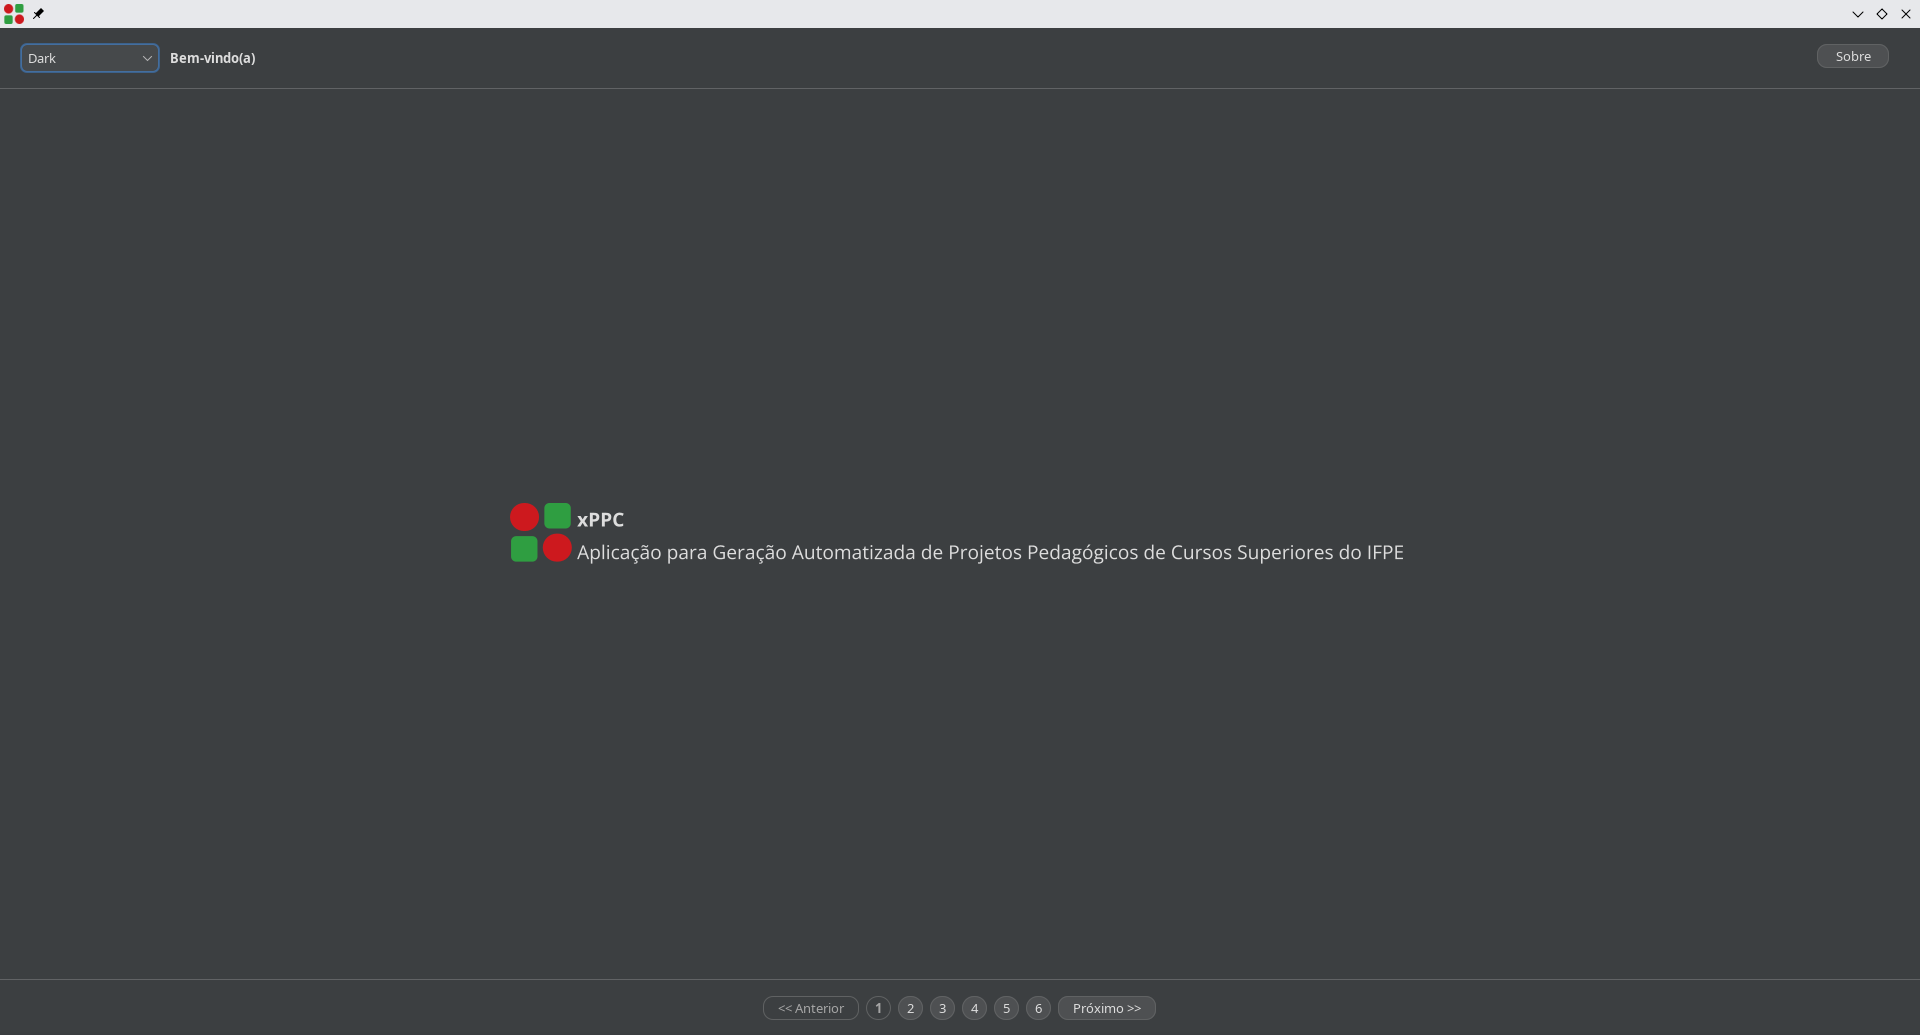
\includegraphics[width=\textwidth]{imagens/cover_dark.png}
        \caption{Tema Escuro (Padrão)}
        \label{fig:capa_dark}
    \end{subfigure}
    \begin{subfigure}{0.9\textwidth}
        \centering
        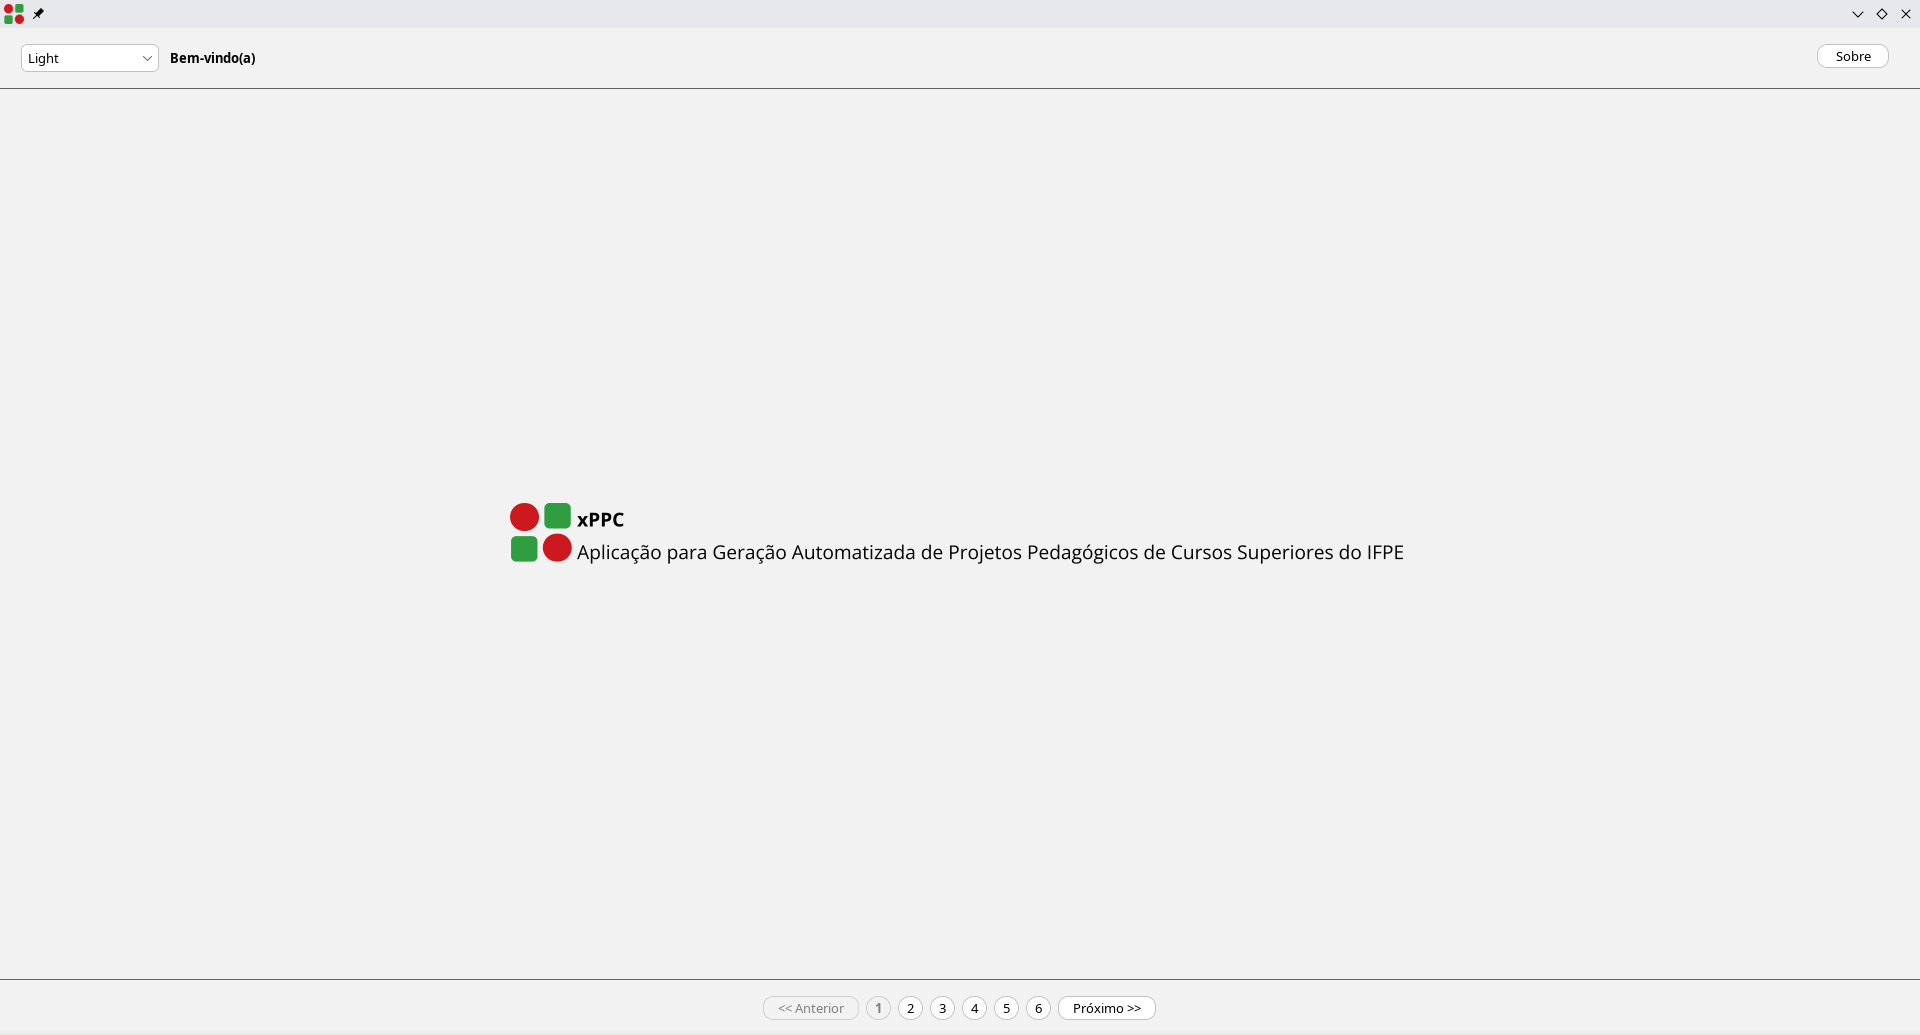
\includegraphics[width=\textwidth]{imagens/cover_light.png}
        \caption{Tema Claro}
        \label{fig:capa_light}
    \end{subfigure}
\end{figure}


\begin{figure}[htb]
    \caption{\label{fig:proponente}Tela de informações da proponente}
    \centering
    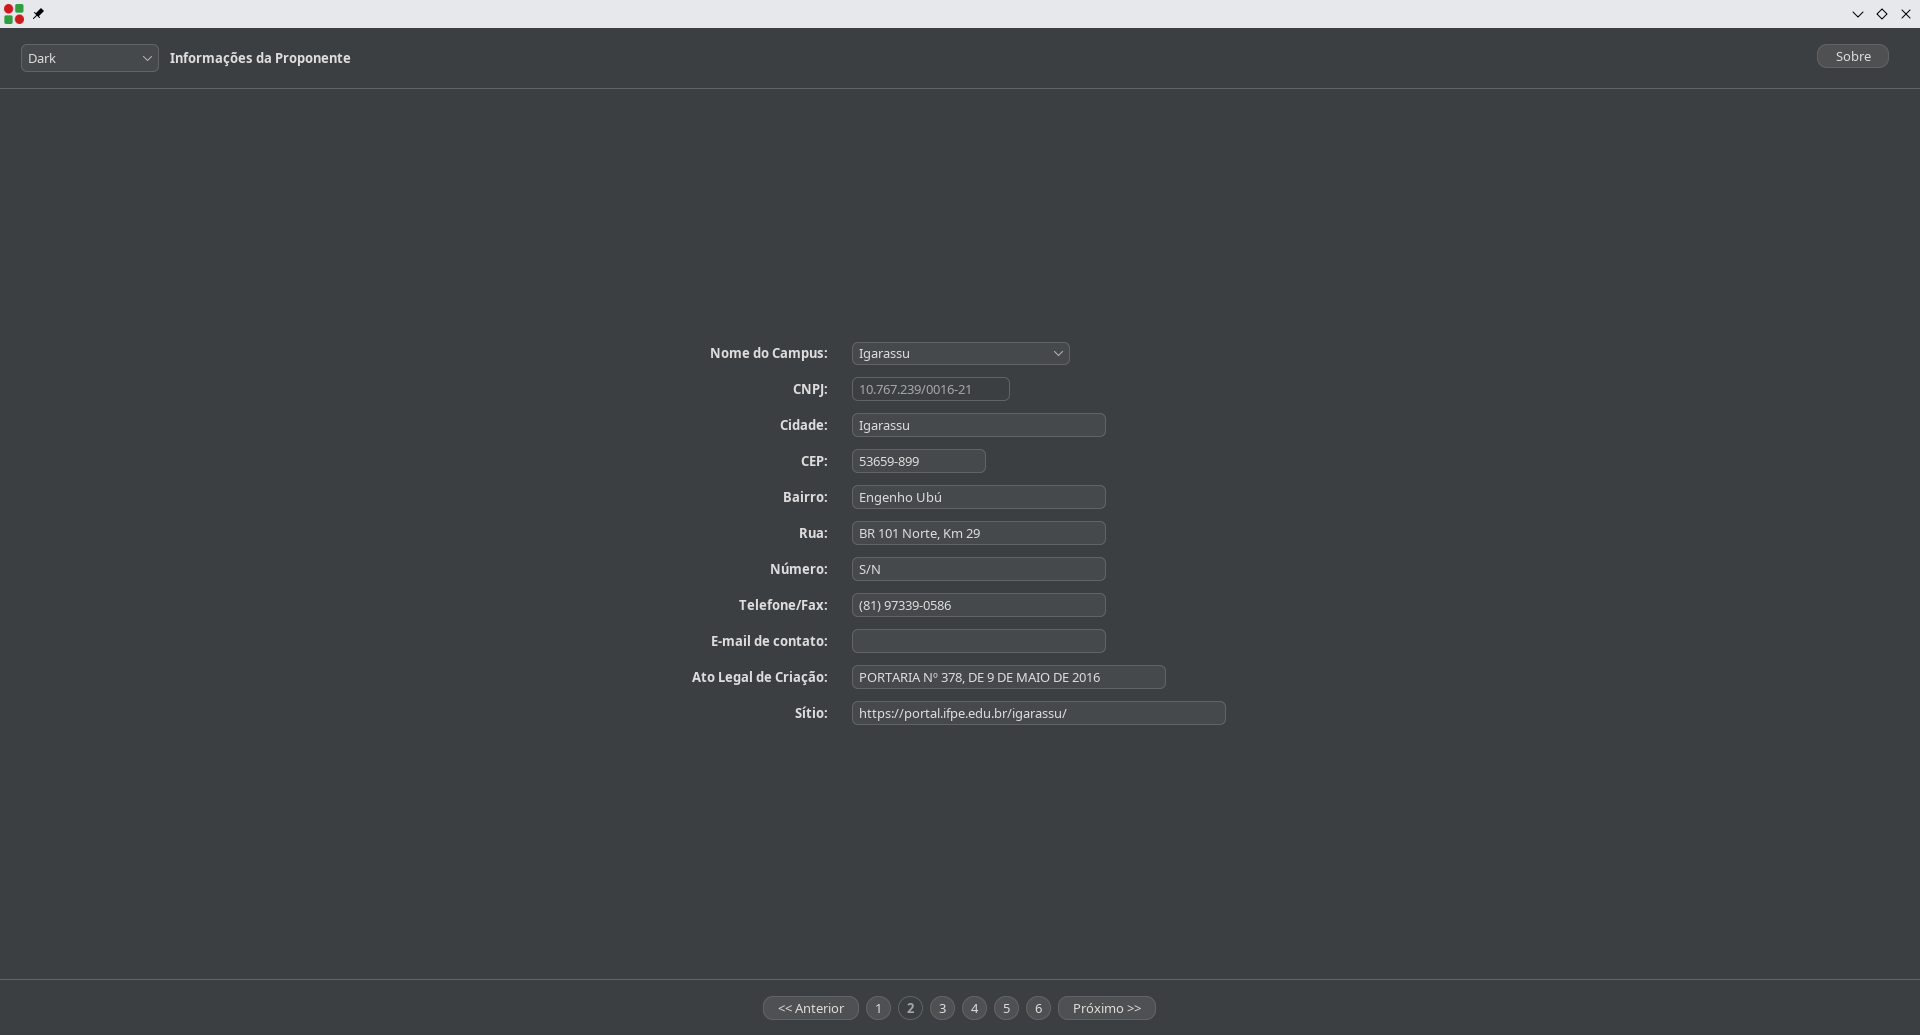
\includegraphics[scale=0.3]{imagens/proponent_dark.png}
\end{figure}

\begin{figure}[htb]
    \caption{\label{fig:curso}Tela de informações do curso}
    \centering
    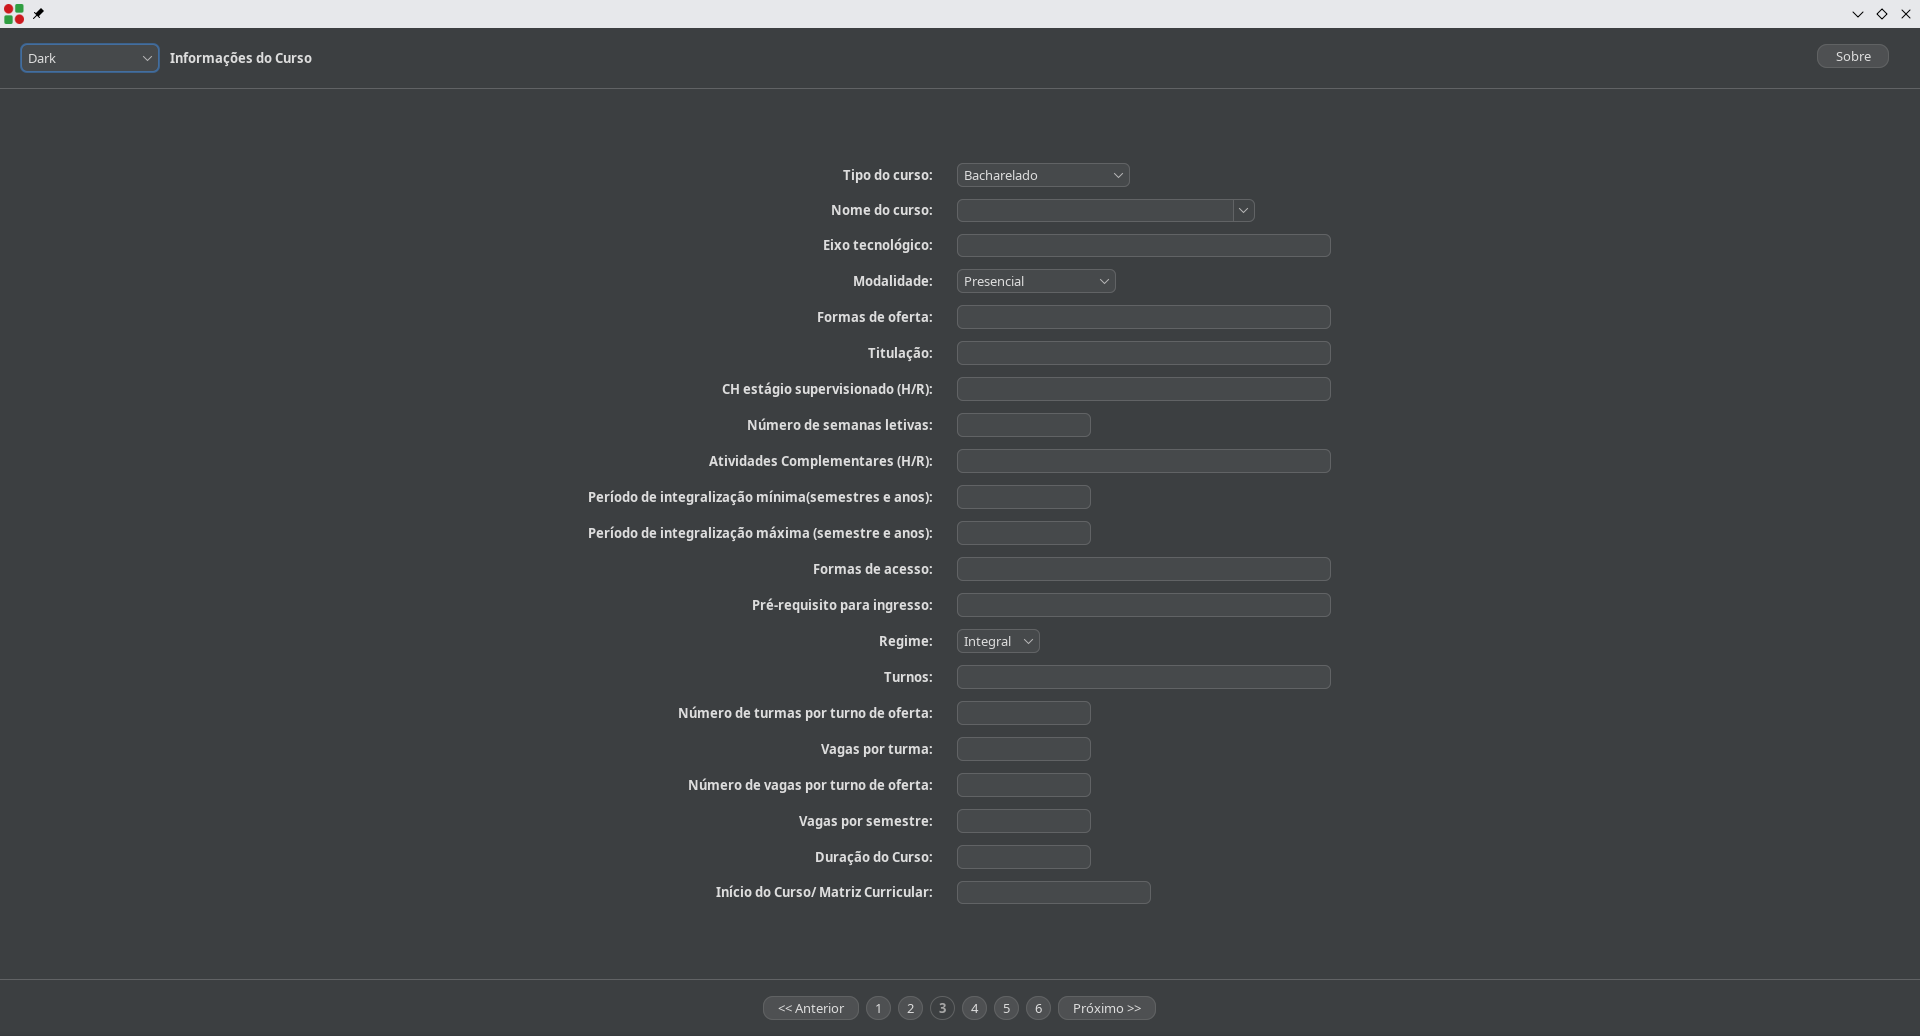
\includegraphics[scale=0.3]{imagens/course_dark.png}
\end{figure}

\begin{figure}[htb]
    \caption{\label{fig:situacao}Tela referente à situação do curso}
    \centering
    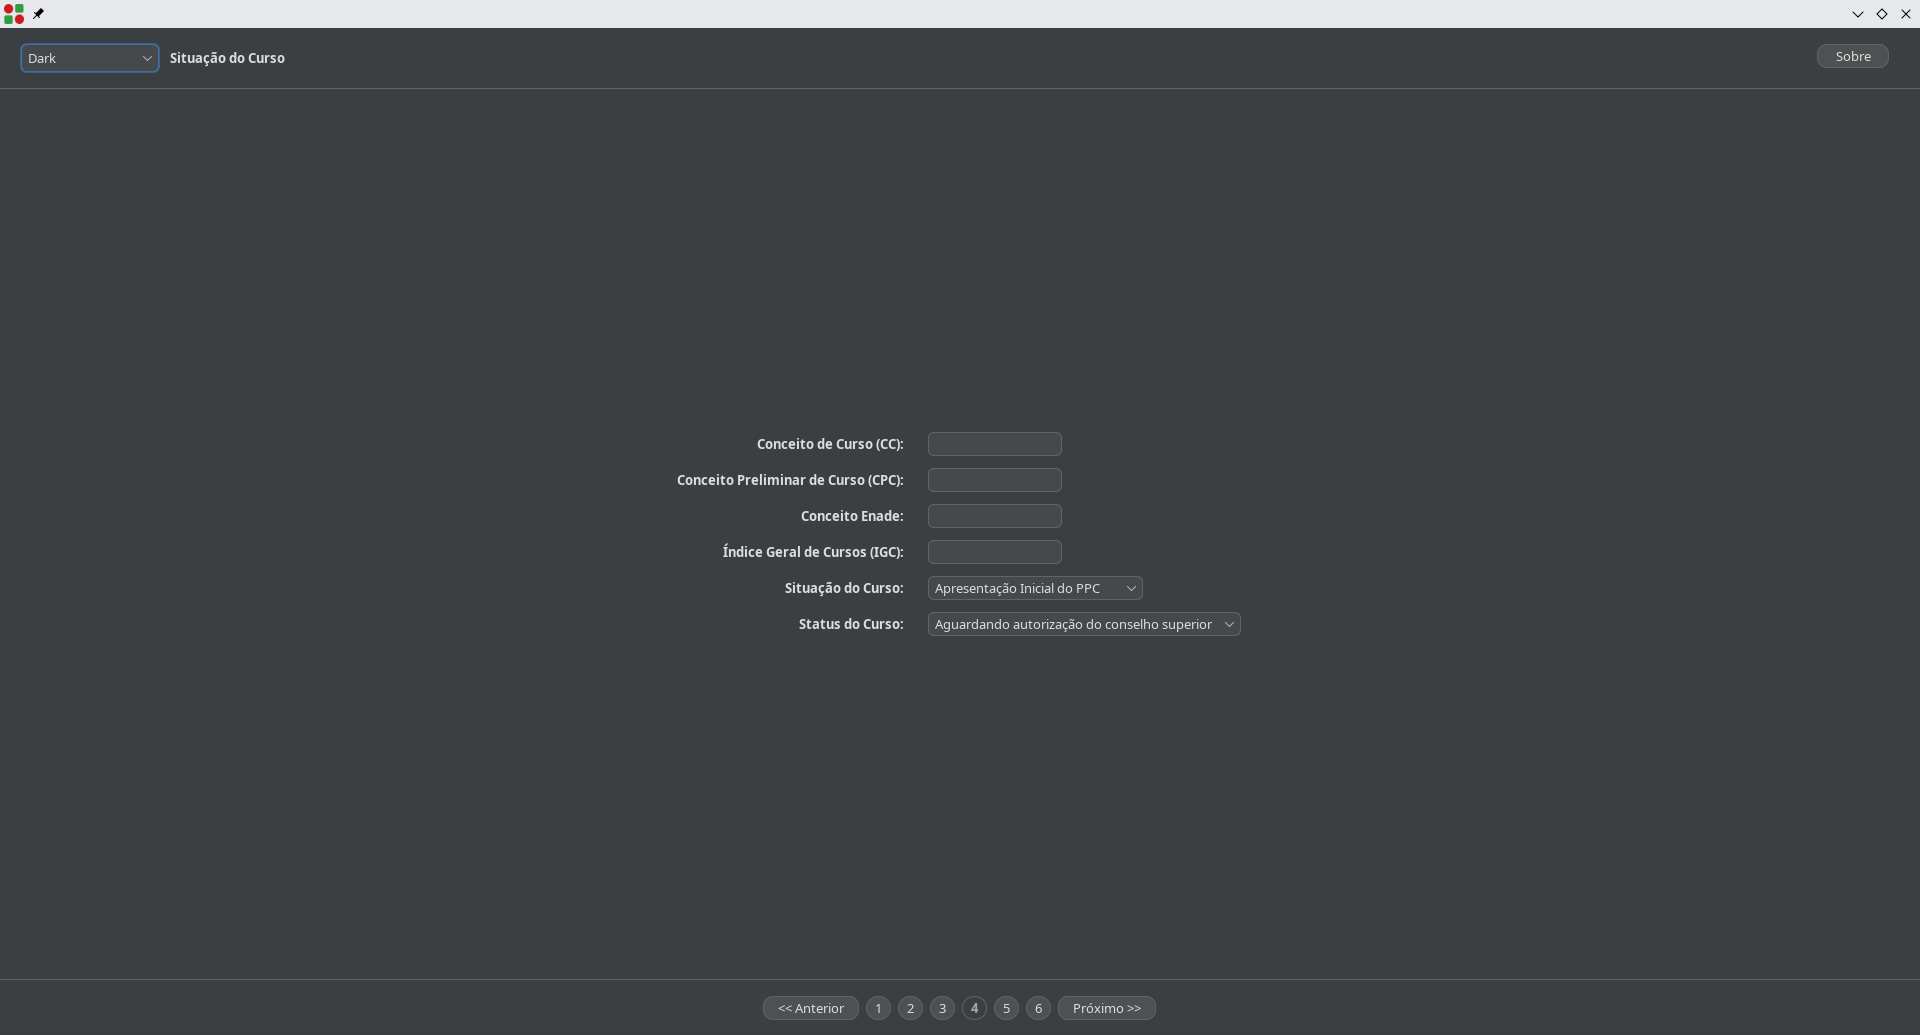
\includegraphics[scale=0.3]{imagens/course_situation_dark.png}
\end{figure}

\begin{figure}[htb]
    \caption{\label{fig:cc}Tela de cadastramento de componentes curriculares}
    \centering
    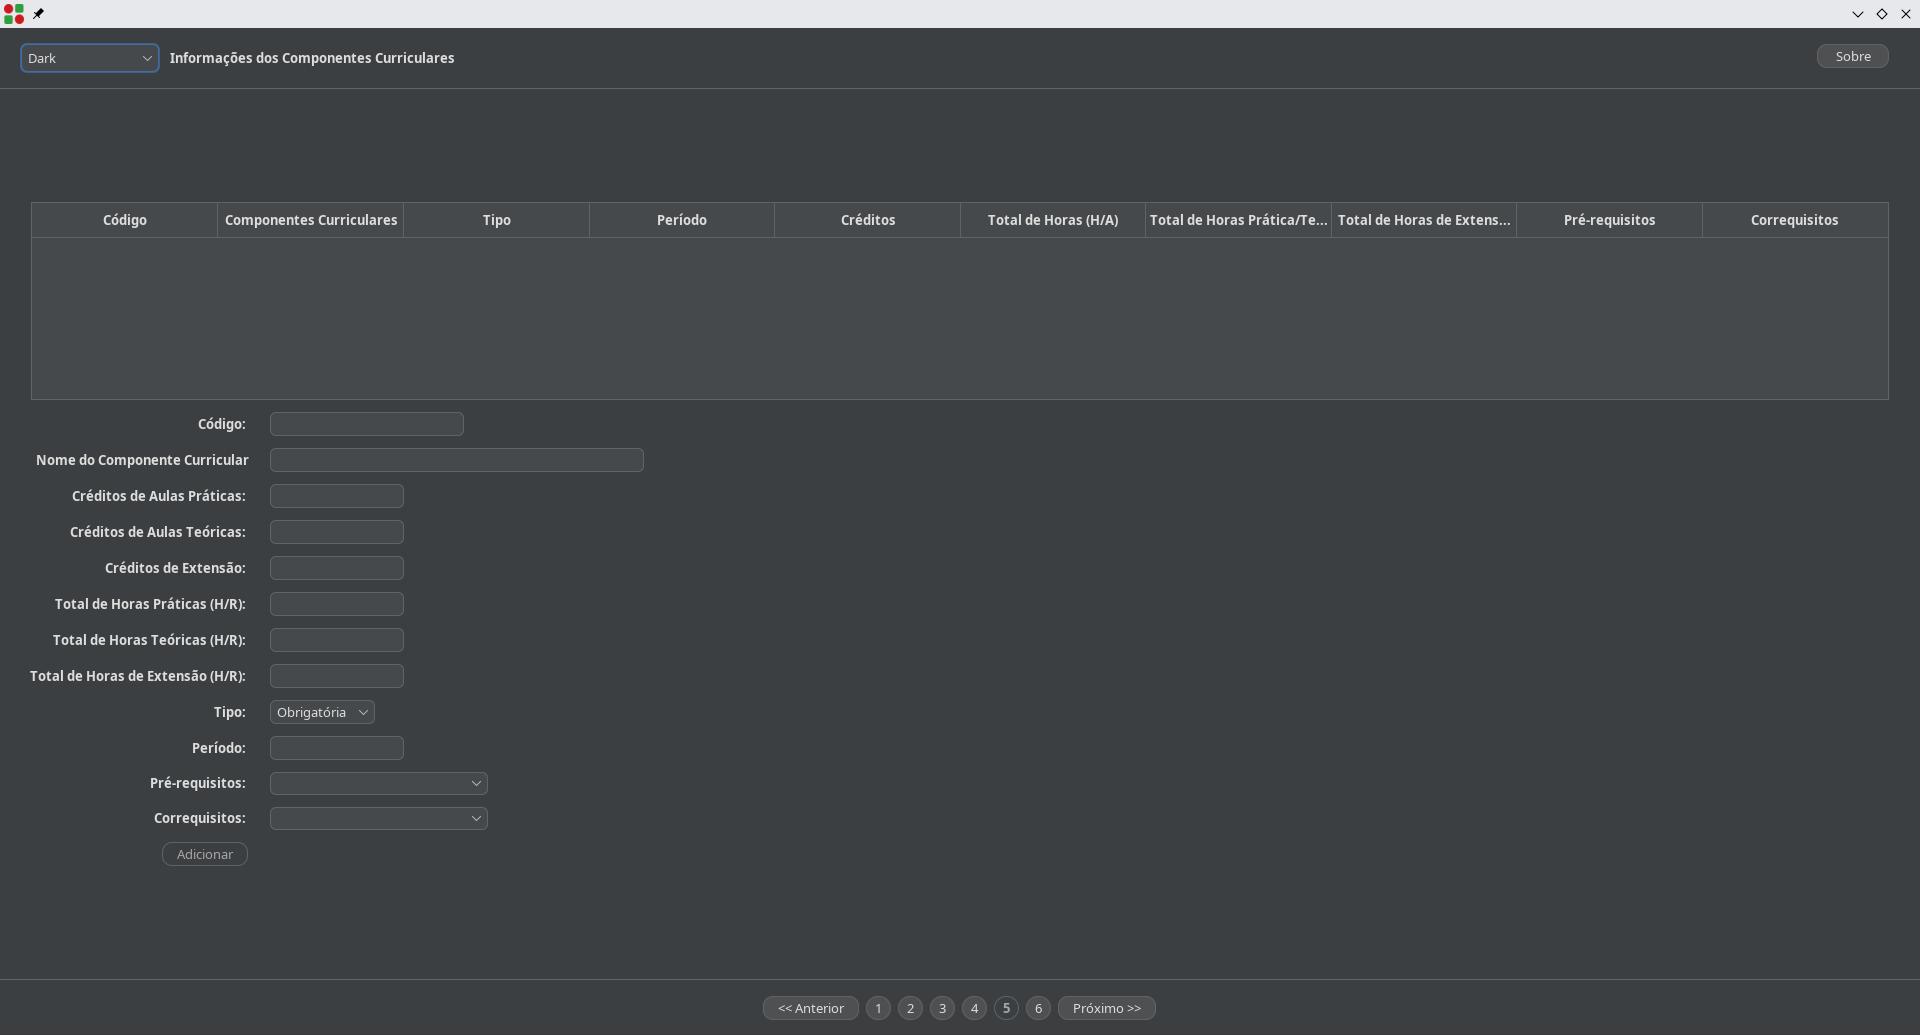
\includegraphics[scale=0.3]{imagens/cc_dark.png}
\end{figure}

\begin{figure}[htb]
    \caption{\label{fig:geracao}Tela final para geração do documento}
    \centering
    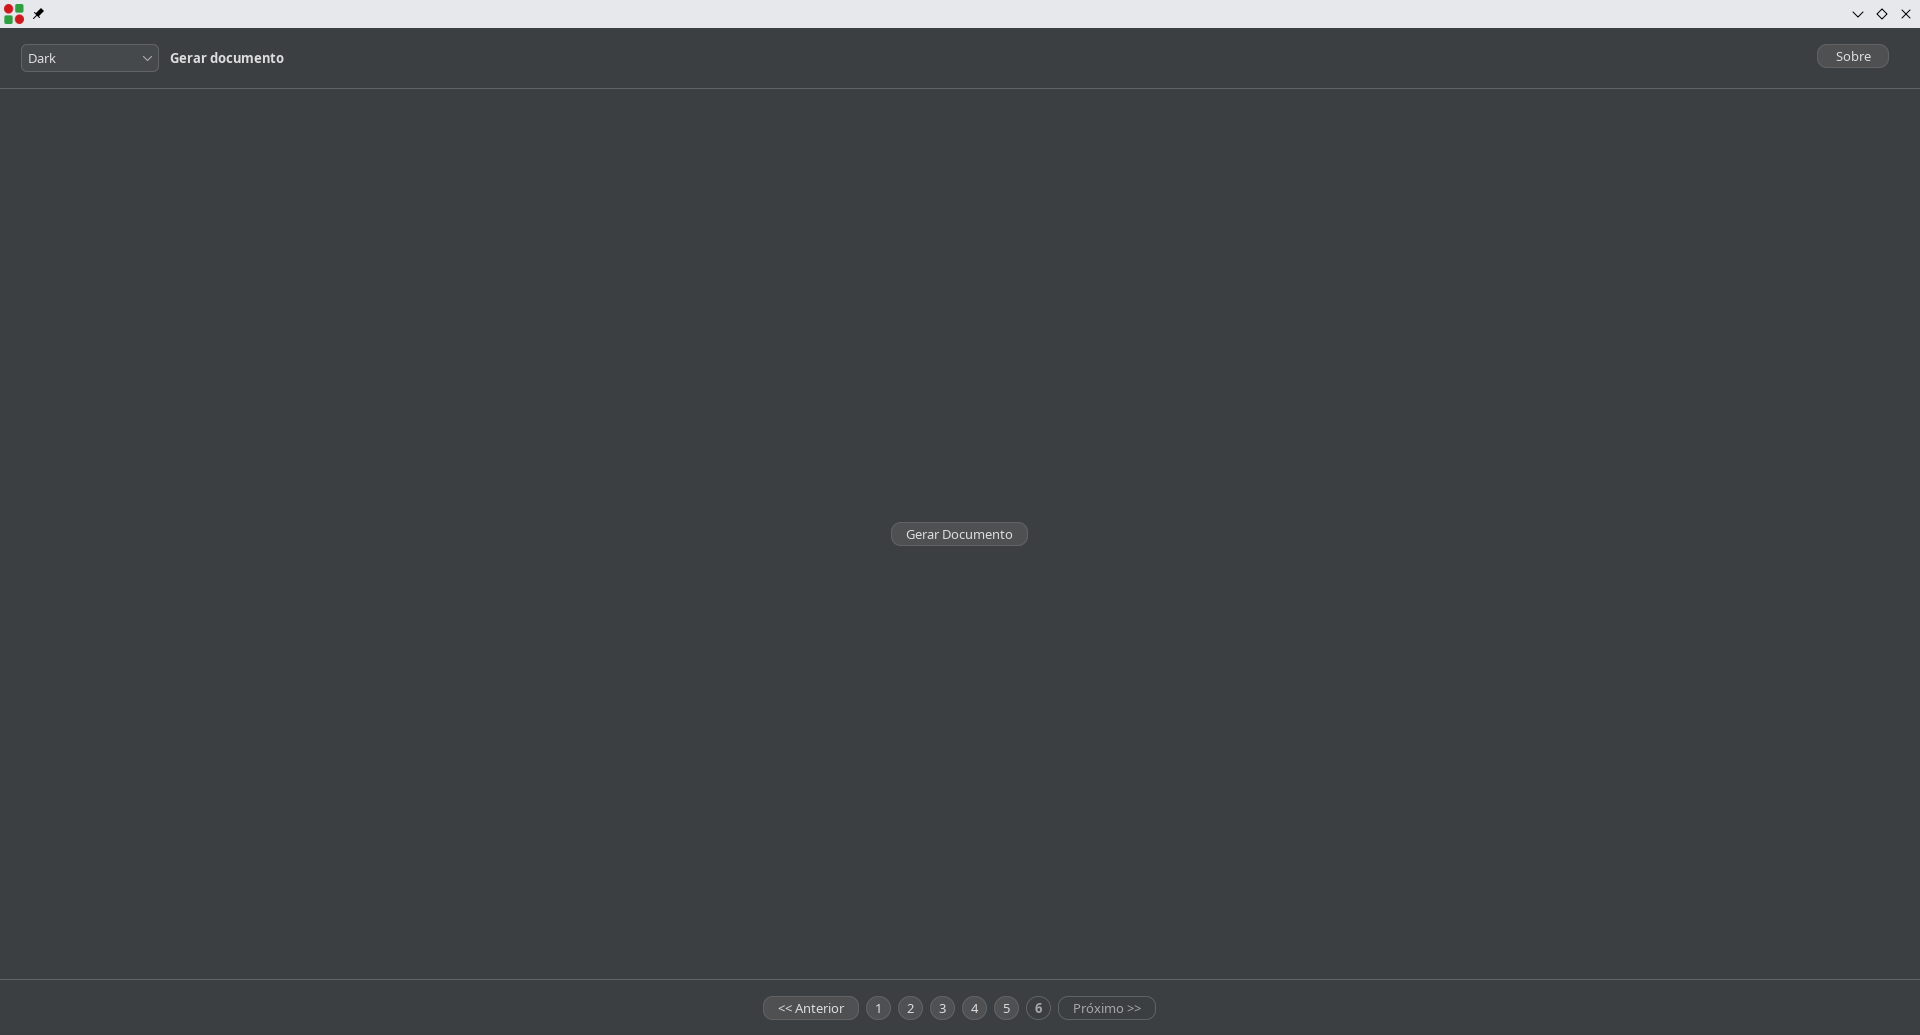
\includegraphics[scale=0.3]{imagens/generation_dark.png}
\end{figure}

\begin{figure}[htb]
    \caption{\label{fig:aviso}Aviso de carga horária insuficiente}
    \centering
    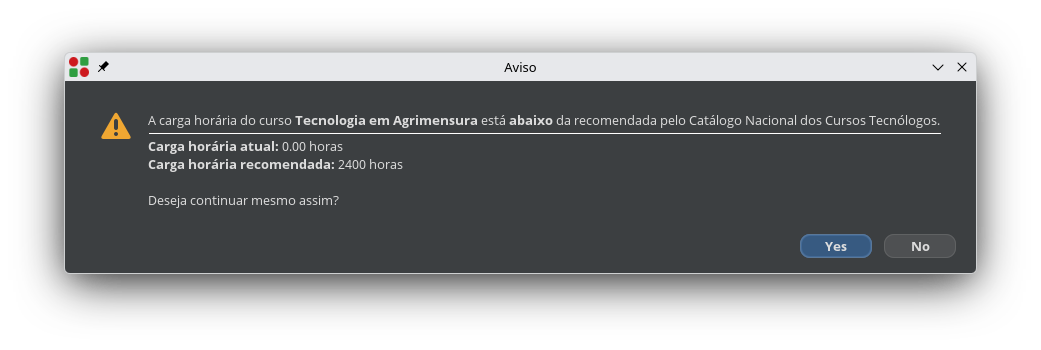
\includegraphics[scale=0.5]{imagens/warning_dark.png}
\end{figure}

\begin{figure}[htb]
    \caption{\label{fig:sucesso}Modal de sucesso}
    \centering
    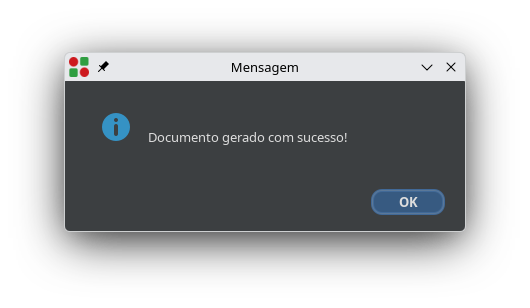
\includegraphics{imagens/success_dark.png}
\end{figure}

\begin{figure}[htb]
    \caption{\label{fig:fluxo_usuario}Fluxo de uso do usuário}
    \centering
    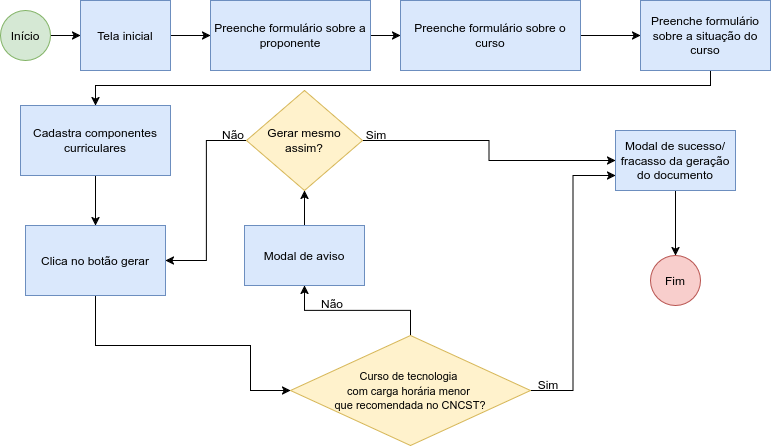
\includegraphics[scale=0.55]{imagens/fluxo_usuario.png}
\end{figure}